Sistem navigasi pada penelitian ini terdiri dari empat subsistem utama yang saling terhubung dalam kerangka kerja ROS2.
Secara garis besar, arsitektur sistem mencakup subsistem persepsi visual untuk segmentasi area jalan, subsistem lokalisasi untuk estimasi posisi kendaraan, subsistem perencanaan navigasi untuk menghasilkan rute lintasan.
Diagram blok keseluruhan sistem ditunjukkan pada Gambar~\ref{fig:diagram_blok}.

\begin{figure}[H]
    \centering
    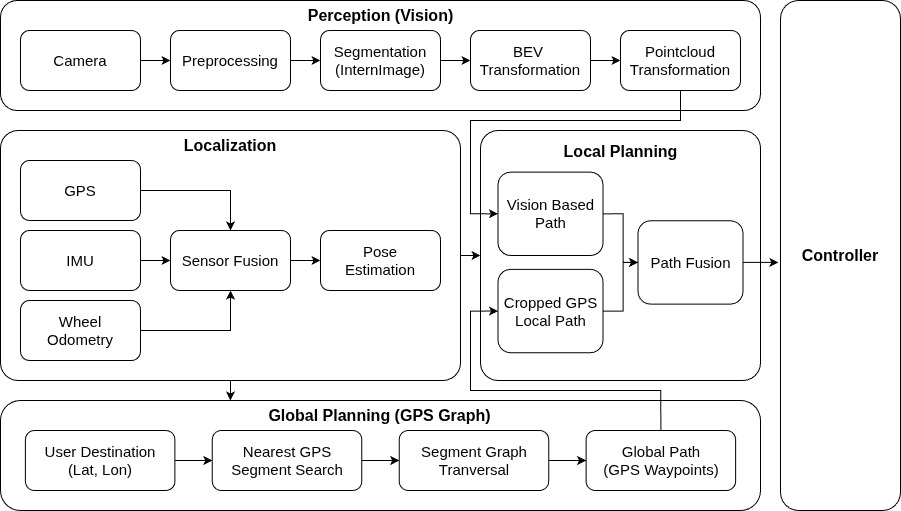
\includegraphics[width=0.95\textwidth]{gambar/diagram_omoda.jpg}
    \caption{Diagram blok arsitektur sistem navigasi.}
    \label{fig:diagram_blok}
\end{figure}